\documentclass[letterpaper]{article} % DO NOT CHANGE THIS
\usepackage[submission]{aaai2027} % DO NOT CHANGE THIS
\usepackage[hyphens]{url} % DO NOT CHANGE THIS
\usepackage{graphicx} % DO NOT CHANGE THIS
\urlstyle{rm} % DO NOT CHANGE THIS
\def\UrlFont{\rm} % DO NOT CHANGE THIS
\usepackage{natbib} % DO NOT CHANGE THIS AND DO NOT ADD OPTIONS
\usepackage{caption} % DO NOT CHANGE THIS AND DO NOT ADD OPTIONS
\usepackage{booktabs}
\usepackage{amsmath}
\frenchspacing % DO NOT CHANGE THIS

\pdfinfo{
/TemplateVersion (2027.1)
}

\setcounter{secnumdepth}{1}

\title{Measure Before You Reuse: Qualifying Computation-Reuse Claims in LLM Agent Workflows}
\author{Anonymous Submission}
\affiliations{}

\begin{document}

\maketitle

\begin{abstract}
Reusing previously completed computation---such as cached tool results, recorded
model responses, or repaired intermediate state---can reduce the cost of LLM
agent workflows. Yet a reuse claim is meaningful only if one can identify
what was delivered, what was actually accessed, which executions were
skipped, at what validation cost, and whether reuse changed the outcome. We
study this measurement problem. First, across three proxy analyses, output
similarity, lexical overlap, and citation mentions did not provide validated
evidence for the equivalence or downstream-dependence claims tested. Second,
we introduce a preregistered evidence ladder that separates non-delivery,
typed projection, and read-level access, and apply it at pinned commits to
AutoGen, LangGraph, and SWE-agent's RetryAgent; within this bounded audit,
none of the located public artifacts provides a qualifying runtime trace for
a strong selective-consumption testbed. Third, we derive a cost model for
speculative reuse that shows that the feasible cost regime depends on
verifier cost and on whether a verifier can distinguish reuse-induced damage
from baseline error. Finally, we specify an outcome-grounded protocol for
measuring realized skips, validation overhead, and outcome agreement, and
apply its static qualification gate, which rejects a proposed testbed as
ineligible under the stated counterfactual and implementation criteria.
Together, these results provide an auditable standard for deciding when an
agent-workflow reuse claim is supported, when it is only code-possible, and
when the available measurement cannot identify the claim.
\end{abstract}

\section{Introduction}

Agent workflows repeatedly produce expensive intermediate artifacts: model
responses, plans, tool results, retrieved evidence, and repaired state. Prior
systems reuse plans, tool calls, prompt prefixes, or speculative work to reduce
latency and cost \cite{agentreuse2024,toolcacheagent2026,kvflow2025,
promptcache2024,sherlock2025,speculativeActions2026}. The engineering question
is often phrased as whether a cache or replay policy obtains a ``hit.'' The
scientific claim is harder. A hit does not establish which consumer received
the artifact, whether that consumer accessed it, whether an underlying
execution was skipped, how much validation cost, whether the final task result
changed, or whether a failure was caused by reuse rather than by the baseline
workflow.

Conflating these claims creates two failure modes. First, an apparently sparse
dependency pattern can be an artifact of a final-text proxy: a consumer may
use an input without copying or citing it. Second, a verifier can correctly
reject a failed task while being unable to attribute that failure to reuse.
The former exaggerates selective-consumption opportunity; the latter can erase
economic benefit by recomputing ordinary baseline failures. These are
identifiability problems: the observed record does not determine the claimed
event.

We ask three research questions. \textbf{RQ1:} Which native records identify
consumption, execution, cost, outcome, and attribution claims? \textbf{RQ2:}
What levels do three text-proxy analyses and three prespecified public-agent
audit units support? \textbf{RQ3:} How do verifier cost and attribution ability
alter the feasible regime for speculative reuse?

We make four contributions. First, we report three bounded failure analyses
showing that output similarity, verbatim overlap, and citation mention did not
validate the particular equivalence or dependence claims for which they were
used. Second, we introduce a prospectively frozen Q0--Q3/QX audit code for
selective consumption, crossed with an independent code-only versus
trace-confirmed evidence axis, and apply it to one native path or fixture in
each of AutoGen, LangGraph, and SWE-agent's RetryAgent. Third, we derive and
instantiate a verifier-aware cost model that separates outcome rejection from
post-hoc reuse-damage attribution. Fourth, we specify an outcome-grounded
actual-skip protocol and execute its static design-qualification gate on a
proposed testbed.
The gate rejects the design before implementation. This paper is therefore a
measurement and methodology study, not a new cache mechanism and not a report
of a new model experiment.

\section{Background and Related Work}

\paragraph{Reuse mechanisms.}
Agent reuse spans several layers. Plan reuse retrieves prior plans before a
new run \cite{agentreuse2024}; Tool Cache Agent caches tool-call results and
models expiration and inter-tool invalidation \cite{toolcacheagent2026}; and
Agent Workflow Memory retrieves procedural workflows rather than completed
computation artifacts \cite{agentWorkflowMemory2025}. At the serving layer,
Prompt Cache and KVFlow reuse prompt-prefix computation
\cite{promptcache2024,kvflow2025}, while editable KV-cache work studies
composable intermediate representations \cite{prefillnotes2026}. These works
show that caching and reuse are established mechanism spaces. We instead ask
what evidence is sufficient for claims made \emph{about} a reuse execution.

\paragraph{Speculation and verification.}
Sherlock combines selective verification, background speculation, and
rollback for agentic workflows \cite{sherlock2025}. Speculative Actions
executes predicted future actions and validates them against an authoritative
action \cite{speculativeActions2026}; StepCache reports step-level retrieval,
lightweight checks, and selective patching \cite{stepcache2026}. Such systems
motivate our cost model, but historical artifact replay raises a distinct
attribution question: a failed final task may have failed even under
from-scratch execution. Outcome checking alone does not isolate reuse-induced
damage.

\paragraph{Dependencies and observability.}
Incremental systems formalize dependency tracking, partial materialization,
and from-scratch consistency \cite{buildsystems2018,noria2018,dbsp2023}.
Agent frameworks, however, often expose rendered messages, shared mutable
state, or application-defined telemetry rather than a stable dependency trace.
Recent work systematizes agent execution provenance and argues that final
answers alone are insufficient \cite{agentTraceProvenance2026}; ProvenanceGuard
uses stable tool/source identities for source-sensitive factuality checks
\cite{provenanceGuard2026}. We do not propose a general provenance taxonomy or
verifier. Our narrower contribution is a reuse-specific decision procedure
that jointly requires consumption, actual skip, validation cost, paired
outcome, and reuse-damage attribution. It is not a new invalidation algorithm.

\paragraph{Outcome-grounded evaluation.}
Stateful tool-use benchmarks such as ToolSandbox provide executable milestone
and failure conditions rather than relying only on answer text
\cite{toolsandbox2025}. Such an oracle can support an outcome claim, but it
does not by itself record whether work was skipped or whether reuse caused a
difference. Our protocol therefore treats a task oracle as one required column
of evidence rather than as a complete reuse evaluation.

\section{Identifiability-First Measurement}

\subsection{Separate the Claim Before Measuring It}

Let a producer create artifact $a$ and let $c$ denote a downstream consumer.
We distinguish five families of claims.

\begin{enumerate}
    \item \textbf{Consumption:} whether $a$ was delivered to $c$, which typed
    projection was delivered, or which records or fields $c$ actually read.
    \item \textbf{Execution:} whether the producer invocation was executed or
    skipped, with a stable identity for the replay source.
    \item \textbf{Cost:} complete-run, replay, and validation work on a common
    cost basis.
    \item \textbf{Outcome:} agreement with a paired from-scratch run under a
    task-native oracle.
    \item \textbf{Attribution:} whether an outcome difference was caused by
    reuse rather than by baseline task error.
\end{enumerate}

These claims are not substitutes. A routing record can identify non-delivery
without proving a skip. An execution bit can prove a skip without showing
outcome agreement. A test oracle can detect failure without identifying its
cause. Figure~\ref{fig:claim-map} summarizes the required separation.

\begin{figure*}[t]
\centering
\small
\setlength{\tabcolsep}{4pt}
\begin{tabular}{p{0.145\textwidth}p{0.145\textwidth}p{0.145\textwidth}p{0.145\textwidth}p{0.145\textwidth}p{0.145\textwidth}}
\toprule
\textbf{Consumption} & \textbf{Execution} & \textbf{Cost} & \textbf{Outcome} & \textbf{Attribution} & \textbf{Evidence status} \\
\midrule
delivery, typed projection, or native read log & invocation ID, replay-source ID, execution flag & verifier and replay work normalized by a full run & paired task-native oracle under changed state & paired baseline label or runtime causal certificate & code path only, or a qualifying serialized runtime instance \\
\bottomrule
\end{tabular}
\caption{Claim-to-record map. The audit code summarizes consumption/access
evidence. Execution, cost, outcome, and attribution require additional records;
CODE\_ONLY and TRACE\_CONFIRMED form an orthogonal evidence-status axis.}
\label{fig:claim-map}
\end{figure*}

\subsection{An Audit Code for Selective Consumption}

Q0--Q2 describe routing structure, Q3 describes read observability, and QX is
a measurement-failure sentinel; they are not mutually exclusive ontological
properties. As a post-audit, verdict-invariant semantic clarification, we use
this precedence to issue one code: assign \textbf{QX} if only a prohibited semantic proxy exists;
otherwise assign \textbf{Q3} when a native field-, record-, or read-level log
binds actual access to stable artifact and consumer identities; otherwise use
\textbf{Q2} for different native typed projections of the same stable artifact,
\textbf{Q1} when native routing withholds it from at least one real consumer,
and \textbf{Q0} when all real consumers receive the same complete artifact.
A Q2 consumer must not retain an unmodeled raw-artifact path. The single label
is therefore an assignment convention; Figure~\ref{fig:claim-map} keeps claim
type and evidence status on separate axes.

Final-text substring, Jaccard similarity, embedding, attention, citation
mention, model self-report, or an LLM judge cannot promote QX to Q1--Q3.

The Q level is crossed with an evidence status. A source path at a pinned
commit is \textbf{CODE\_ONLY\_CANDIDATE}. It becomes
\textbf{TRACE\_CONFIRMED} only when at least one public serialized runtime
instance binds the native mechanism to stable producer-artifact and consumer
identities. Test source, documentation, a final answer, or a log without these
bindings does not suffice.

For a strong selective-consumption testbed we further require Q2 or Q3,
TRACE\_CONFIRMED evidence, at least two real downstream consumers,
independently reconstructable consumer inputs, complete accounting for raw
bypasses, and an outcome oracle available in principle. Meeting this full
conjunction would qualify a testbed; it would not establish that a reuse method is safe or
beneficial.

\subsection{Operational Identification and Downgrading}

We use \emph{identify} in an operational sense. Given an archived record, an
independent parser must be able to reconstruct the claimed event without
running the studied model and without interpreting the semantics of its final
answer. For delivery this requires an artifact ID, a consumer ID, and the
serialized payload or projection. For read access it additionally requires a
record/field key emitted by the execution mechanism. For a skip it requires an
invocation ID, a replay-source ID, and an execution flag. Outcome and
attribution then require paired task IDs and oracle values. This definition is
a reproducible sufficiency test for the present protocol; we do not claim it is
the only philosophically possible account of model use.

Four downgrade rules make the test conservative. First, source support without
a qualifying instance is code-only, even when the call chain is unambiguous.
Second, a consumer's unlogged raw-artifact path blocks Q2 because the visible
projection need not be its complete input. Third, absent stable parent identity
prevents combining two records into ``projections of the same artifact.''
Fourth, outcome failure without a paired baseline cannot be labeled
reuse-induced damage. These rules deliberately preserve ``unresolved'' rather
than converting missing evidence into a negative mechanism claim.

\subsection{Prospectively Frozen Audit Procedure}

The selective-consumption audit used the following decision procedure.

\begin{enumerate}
    \item Freeze two or three candidates, their structural rationale, and the
    Q definitions before deep source review or candidate-specific results.
    \item Pin each source repository and locate artifact creation, routing or
    projection, consumer-input assembly, raw bypass, access logging, and trace
    serialization.
    \item Search only existing public traces, event logs, test artifacts, and
    example runs; do not generate a trajectory or modify instrumentation.
    \item Bind any candidate runtime instance to stable producer and consumer
    identities. If binding fails, retain static facts but leave trace-derived
    counts undefined.
    \item Assign exactly one reported Q code under the prespecified
    highest-level rule and a separate evidence status, then apply the
    strong-testbed conjunction without adding a fourth
    candidate after seeing the result.
\end{enumerate}

This separation of protocol, uninterpreted results, and verdict was also
enforced in version control. It prevents a promising source path from changing
the measurement definition after inspection. We use ``preregistered'' in the
submitted abstract only in this narrow sense of prospective version-control
freeze, not to imply an external public registry. Likewise, ``standard'' there
means an auditable decision protocol, not a universally validated standard.

\section{Applying the Framework}

\subsection{Why Three Text Proxies Did Not Identify the Claim}

Table~\ref{tab:proxies} reanalyzes three bounded uses of final-text signals.
The analyses target different estimands and are not independent replications.
Their common result is narrower: the observed proxy did not validate the
claim for which it had been used.

The first is a post-hoc diagnostic of 18 frozen agent runs. It examines eight
events admitted only by an uncalibrated diff cutoff and follows each event at
progressively stricter units: next action, complete invocation, suffix, and
exit status. The second uses 100 frozen multi-stage traces. Its unit is one of
4,968 non-system artifact--consumer edges; ``use'' is either verbatim
substring overlap or 3-gram Jaccard overlap of at least $0.5$. The third uses
1,000 document-perturbation/consumer pairs and marks use when the output cites
the document title. It compares this mark with a downstream repair flip. None
of these designs instruments what the consumer actually received or read.

\begin{table*}[t]
\centering
\small
\setlength{\tabcolsep}{4pt}
\begin{tabular}{p{0.17\textwidth}p{0.17\textwidth}p{0.28\textwidth}p{0.28\textwidth}}
\toprule
\textbf{Target claim} & \textbf{Observed proxy} & \textbf{Observed behavior} & \textbf{Admissible conclusion} \\
\midrule
Safe equivalence of adjacent invocations & uncalibrated output diff and command similarity & All 8 candidate events came from parent-directory mtime artifacts; 6/8 disagreed at the next step, 8/8 over the suffix, and 4/8 differed in exit status (patch correctness was unavailable). Requiring full-invocation identity reduced the signal to zero. & The tested cutoff did not identify safe invocation equivalence. This does not show that exact reuse never occurs. \\
Downstream use of a sentence region & substring and $0.5$-threshold Jaccard overlap & Across 4,968 producer--consumer edges, the zero-use fraction was 98.09\% for substring and 95.69\% for Jaccard; both median and 90th percentile were zero. & The measure was degenerate on these traces. Zero copied text is not evidence of no access or dependence. \\
Downstream use of a document & title/citation mention in final output & In 1,000 perturbation pairs, 53 cited pairs had 0 flips and 947 uncited pairs had a 5.07\% flip rate; the observed contrast was exploratory and underpowered in the cited stratum. & Mention was not a validated usage oracle and cannot determine the causal direction of a flip. \\
\bottomrule
\end{tabular}
\caption{Bounded proxy analyses. Each conclusion is restricted to the tested
proxy and estimand; none supports a universal claim about whether an LLM used
text.}
\label{tab:proxies}
\end{table*}

The first analysis also exposed a unit-label mismatch: a predicate named for
byte-exact reuse required node text to differ. Correcting it found no hit in
that six-task slice, without supporting a general claim about reuse frequency.

The second analysis computed large apparent invalidation savings precisely
because almost every consumer output copied none of the candidate sentence.
Interpreting those zeros as non-use would assume the conclusion. The third
analysis has the same problem at document granularity: a title can be omitted
after substantive use, while a mention can occur without causal dependence.
We therefore exclude all three signal families from the selective-consumption
ladder.

The failures have different diagnoses. The diff analysis combines a
\emph{unit error} (command fragment versus complete invocation) with an
environmental artifact. The overlap analysis exhibits \emph{construct
collapse}: its mass at zero makes apparent sparsity nearly automatic. The
citation analysis has \emph{causal ambiguity}: mention is neither necessary
nor sufficient for dependence, and its 5.07\% non-mentioned flip rate was not
paired against the 4.7\% identity-control repair rate from the same task
family. Grouping them as ``proxy failures'' is useful for measurement design,
but their different causes are why we do not treat them as replications or
pool their statistics.

\subsection{Pinned Native-Path Audit}

On July 22, 2026, we froze six prescreened systems: three audit units were
included and three excluded with recorded reasons before deep source review or
Q assignment. The included units were an AutoGen handoff example
\cite{autogen2024}, a LangGraph two-consumer fixture \cite{langgraphRepo}, and
SWE-agent RetryAgent's optional Preselector path \cite{sweagent2024}. They span
native message routing, graph state flow, and a multi-attempt controller. Each
repository was pinned to an immutable commit. We located artifact creation,
routing or projection, consumer-input assembly, raw bypass, logging, and trace
serialization without executing a framework, adding telemetry, rewriting
prompts, or inferring access from final text.

Audit units had to be open source, pinnable, agent-workflow relevant, and
auditable without model execution. Each also needed either a producer with at
least two downstream consumers or a native field/read log, plus some public
example, test artifact, or trace whose qualification could be checked. We
searched the pinned repositories, their committed tests/examples, official
documentation, and linked public trajectories available at freeze time.
Systems with a single consumer, paper-only diagrams, or a requirement to add a
reviewer or rewrite a prompt were excluded during prescreening.

For each audit unit we recorded 25 fields, including the complete consumer
input, stable identity, projection type, raw bypass, access log, source
locators, minimum public instance, possible outcome oracle, and integration
cost. Two classes of count are intentionally distinct. A static source locator
can establish that a branch or subscriber exists. Producer-artifact,
consumer-edge, and repeated-consumer counts, however, are runtime quantities;
they remain \emph{undefined}, not zero, when no qualifying instance exists.
Only the qualifying-machine-readable-trace count can be zero after a completed
search of the located artifacts.

Table~\ref{tab:audit} reports the strongest support. ``Qualifying trace = 0''
does not mean that a project has no public logs. It means that none of the
located public artifacts binds the audited mechanism to the stable producer
and consumer identities required by the frozen protocol.

\begin{table*}[t]
\centering
\small
\setlength{\tabcolsep}{4pt}
\begin{tabular}{p{0.115\textwidth}p{0.18\textwidth}p{0.18\textwidth}p{0.13\textwidth}p{0.13\textwidth}p{0.13\textwidth}}
\toprule
\textbf{Audit unit} & \textbf{Native path} & \textbf{Raw bypass / identity} & \textbf{Qualifying runtime trace} & \textbf{Level} & \textbf{Outcome oracle} \\
\midrule
AutoGen handoff example & topic subscription withholds a complete \texttt{UserTask} from nonmatching agents & absent for nonmatching agents; runtime UUID is not bound to a public delivery record & 0 & Q1 / code only & no native deterministic sample oracle \\
LangGraph two-consumer fixture & broadcasts the same full state; custom \texttt{Send.arg} exists elsewhere & shared-state read closure is present and not read-logged & 0 & Q0 / code only & application-defined in principle \\
RetryAgent optional Preselector & withholds unselected submissions from Chooser & controller retention is modeled; no independent artifact UUID in a public instance & 0 (22 tracked trajectories are non-RetryAgent) & Q1 / code only & SWE-bench-style evaluation in principle \\
\bottomrule
\end{tabular}
\caption{Qualification matrix for three prespecified native paths. ``Code
only'' means source support without a qualifying serialized runtime instance;
trace count zero is not a framework-wide no-trace claim. Commits are AutoGen
\texttt{027ecf0}, LangGraph \texttt{31f90df}, and SWE-agent
\texttt{3ea751c}. Static topology is not counted as runtime coverage.}
\label{tab:audit}
\end{table*}

\paragraph{AutoGen: Q1/code only.}
The audited handoff application registers three topic-isolated consumers. A
task sent to an agent-specific topic is delivered only to the matching
subscriber; the selected handler receives the complete task. This is native
non-delivery, not a typed projection. The runtime creates a message UUID, but
the located public event record omits that UUID and does not bind publication
to a receiver. Source therefore supports Q1, while the public artifacts do not
support TRACE\_CONFIRMED.

\paragraph{LangGraph: Q0/code only.}
The runtime can schedule a named node with \texttt{Send(node,arg)}, and
\texttt{arg} becomes the task input. A single destination, however, does not
establish that some other real downstream consumer was denied the same
artifact. The concrete two-consumer fixture sends identical full state to both
retrievers. Moreover, tasks receive a shared-state read closure and the
prebuilt tool path can hydrate full state, with no field-level access log.
This leaves the concrete evidence at Q0.

\paragraph{RetryAgent: Q1/code only.}
A completed attempt normally goes to either a score reviewer or a chooser;
these are alternatives, not two consumers of one artifact. The optional
Preselector path does create Q1 structure: it consumes eligible submissions
and the Chooser receives only the selected subset. The shipped configuration
does not enable that path, and none of 22 tracked trajectories is a RetryAgent
run. Configurable Jinja text rendering is not a typed projection.

\paragraph{Adjudication and negative controls.}
The audit retained public artifacts that failed qualification instead of
discarding them. AutoGen's committed handoff history contains application
state but no message-ID-to-recipient binding. LangGraph's debug and map-reduce
test expectations corroborate source behavior but use placeholder identities
or omit serialized task records. SWE-agent's 22 tracked trajectories provide a
negative control: none contains the RetryAgent reviewer/chooser keys. These
artifacts justify a completed search of the located sources, but not runtime
coverage. For each audit unit, the coordinating reviewer independently checked
at least two load-bearing locators spanning routing and consumer-input
assembly; source interpretations were resolved against the pinned code rather
than by voting across auditors.

No audit unit reaches Q2/Q3 or TRACE\_CONFIRMED, so the strong testbed is
\emph{not found within this bounded audit}. The AutoGen handoff example and
RetryAgent Preselector still show that weak routing-aware non-delivery is
code-possible. Natural selective consumption, stronger typed contracts, and
native read-level evidence remain unresolved outside these paths.

\subsection{Decision Consequences and Falsifiability}

The protocol maps evidence levels to different research claims. A Q1 result
can support context non-delivery or weak selective invalidation, but not
receiver-conditioned validity. Even a trace-confirmed Q2/Q3 result would only
qualify a testbed; efficacy requires a new protocol. With only Q0/Q1 or
code-only results, the prespecified rule stops instead of adding candidates
after the negative result.

The judgments remain falsifiable. An AutoGen export binding runtime UUID,
payload, and recipient could trace-confirm Q1. LangGraph would need a stable
parent ID, two consumer IDs, different serialized projections, and a removed
or logged shared-state read closure for Q2/Q3. A Preselector-enabled RetryAgent
run with stable submission/consumer IDs could trace-confirm Q1; rendered text
would still not be a typed projection.

None of these records would attribute failure to reuse rather than a
from-scratch error. The audit identifies no deployable directed verifier:
selective routing and reuse-damage certification are separate prerequisites.

\section{Verifier-Aware Reuse Economics}

Routing evidence does not establish economic benefit. We use a one-shot,
compute-only additive model and normalize one complete from-scratch execution
to $C_{\mathrm{full}}=1$. Let $s$ be the logical-work fraction initially
avoided, $v=C_{\mathrm{verifier}}/C_{\mathrm{full}}$ the validation cost,
$\rho$ the rejection-and-recompute rate, and $RB$ a fixed rollback overhead.
The verifier is treated as a perfect binary decision rule for whichever label
is substituted. The model excludes the utility cost of a wrong answer,
wall-clock overlap, and serving-system effects. The speculative cost and saving
are

\begin{align}
C_{\mathrm{spec}} &= (1-s)+v+\rho(s+RB), \\
\frac{\Delta}{C_{\mathrm{full}}} &= s-v-\rho(s+RB).
\end{align}

The denominator is a complete baseline run. Thus $v=0.1$ means that validation
costs 10\% of the full execution, not 10\% of the avoided subgraph.

We instantiate the model on 164 archived paired code-repair records. Every task
has a from-scratch baseline and two historical intervention labels, called
reuse and repair, joined by pair ID. The recorded normalized-FLOPs proxy gives
$s=1-\operatorname{mean}(C_{\mathrm{arm}}/C_{\mathrm{full}})$: $0.1440$ for
reuse and $0.1224$ for repair. These are logical-work proxies, not realized
skips or timings. We fix $RB=0.01$ as specified by the protocol. A benchmark
outcome oracle rejects at $\rho_{\mathrm{outcome}}=0.3963$ and $0.3902$. A
paired post-hoc label identifies reuse-induced damage at
$\rho_{\mathrm{blame}}=0.0427$ for both arms; it requires the corresponding
from-scratch baseline outcome and is not available as a runtime certificate.

The paired labels induce four outcome categories. Baseline-correct/arm-wrong
cases are the post-hoc reuse-damage set; baseline-wrong/arm-correct cases are
rescues; both-wrong cases are remaining baseline errors; and both-correct cases
agree successfully. In the reuse arm, 65/164 outputs are wrong, but only 7/164
are baseline-correct/arm-wrong; 58/164 remain wrong when the baseline is also
wrong, and 2/164 are rescues. For repair the corresponding counts are 64, 7,
57, and 3. Thus $\rho_{\mathrm{outcome}}$ equals damage plus remaining error,
whereas $\rho_{\mathrm{blame}}$ retains only the damage cell.

Solving for the largest verifier cost with nonnegative saving gives

\begin{equation}
v^{*}=s-\rho(s+RB).
\end{equation}

Table~\ref{tab:economics} makes the conditional regime explicit. The post-hoc
rows are counterfactual economic analyses, not measurements of a deployable
verifier.

\begin{table}[t]
\centering
\small
\setlength{\tabcolsep}{4pt}
\begin{tabular}{lrr}
\toprule
\textbf{Rejection regime} & \textbf{Reuse $v^{*}$} & \textbf{Repair $v^{*}$} \\
\midrule
Benchmark outcome oracle & 8.3\% & 7.1\% \\
Blame (paired post-hoc only) & 13.7\% & 11.7\% \\
\bottomrule
\end{tabular}
\caption{Verifier-cost break-even fractions of a complete run on the archived
164-task trace set.}
\label{tab:economics}
\end{table}

The stored post-hoc uncertainty intervals use 2,000 task-pair bootstrap resamples, percentile
endpoints, and fixed seed 1. For reuse, the 95\% intervals are $[0.323,0.470]$ for
$\rho_{\mathrm{outcome}}$ and $[0.012,0.079]$ for
$\rho_{\mathrm{blame}}$; the corresponding repair intervals are
$[0.317,0.463]$ and $[0.012,0.079]$. Because $v^{*}$ decreases monotonically
with $\rho$, mapping those endpoints through the cost equation gives outcome
break-even intervals 7.2--9.4\% (reuse) and 6.1--8.0\% (repair). The
post-hoc intervals map to 13.2--14.2\% and 11.2--12.1\%. These intervals condition on the
archived logical-work estimates $s$ and the protocol-fixed assumption $RB$;
they do not include timing or
serving-system uncertainty.

At $v=0.01$, outcome rejection yields net savings of 7.30\% (reuse) and 6.07\%
(repair) of a full run. At $v=0.10$, the signs reverse to $-1.70$\% and
$-2.93$\%. Substituting the post-hoc blame rate would yield $+3.74$\% and
$+1.67$\% at $v=0.10$, but no corresponding deployable directed verifier was
found. Figure~\ref{fig:economics} shows the complete sign map. Thus the
conditional positive regime requires a new deployable directed verifier; it
is not a claim of deployed savings.

\begin{figure*}[t]
\centering
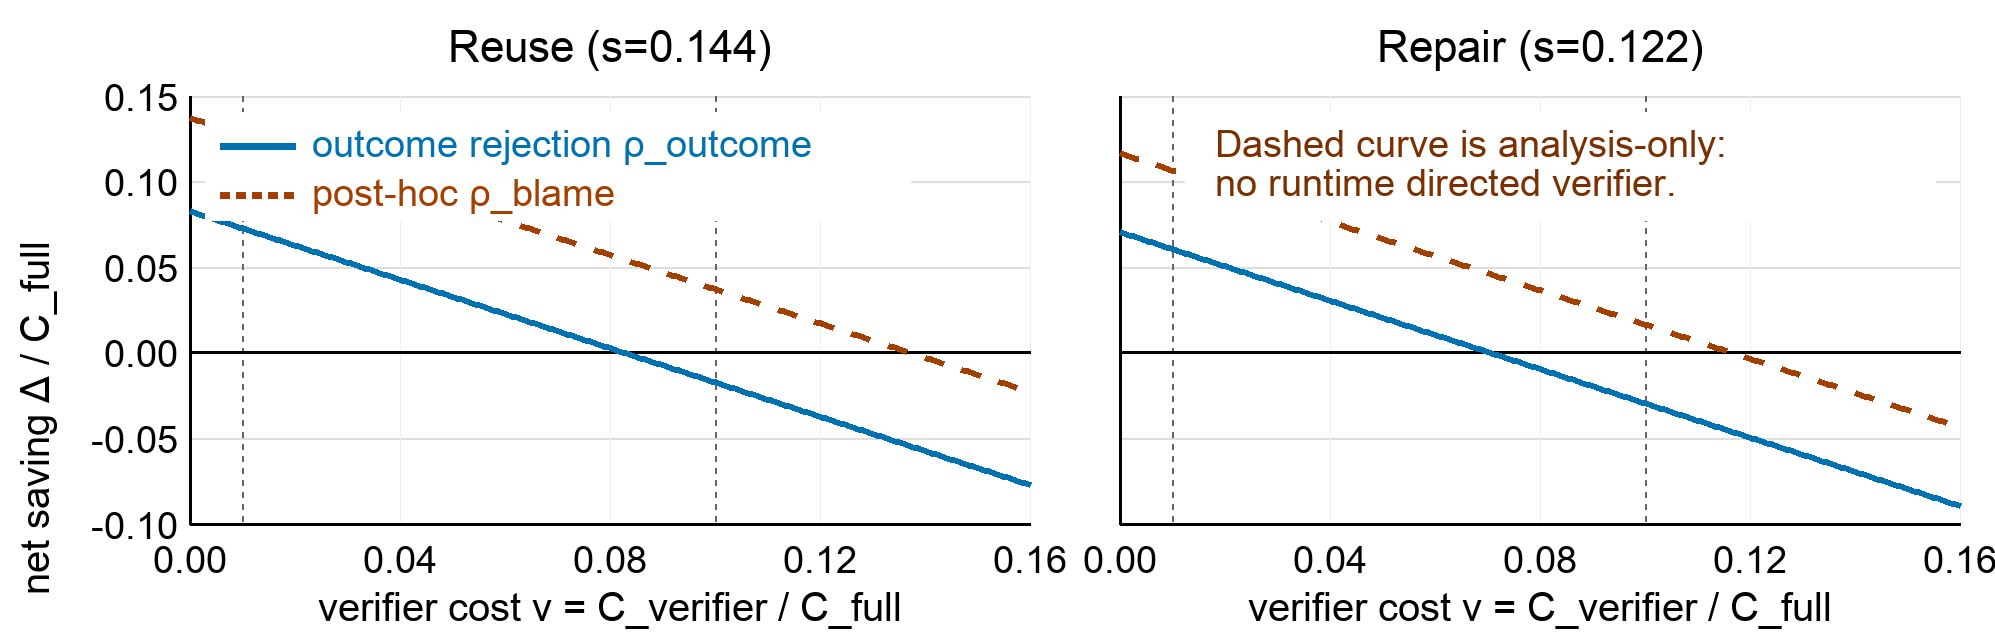
\includegraphics[width=0.95\textwidth]{figures/verifier_cost_sign_map.png}
\caption{Verifier-cost sign map for 164 archived code-repair pairs. Solid
curves use the benchmark-executable outcome-oracle rejection rate. Dashed
curves substitute a post-hoc
reuse-damage rate that depends on paired baseline labels; no runtime directed
verifier realizes that curve. Vertical guides mark $v=0.01$ and $v=0.10$.}
\label{fig:economics}
\end{figure*}

Why is the gap large? Outcome verification rejects both reuse-induced failures
and tasks that the baseline already failed. Recomputing the latter cannot
repair the cause attributed to reuse. The trace pairs also contain rescues:
reuse and repair succeed where the baseline fails in 1.22\% and 1.83\% of
tasks. A verifier that simply demands success discards this causal structure.
A useful directed verifier would need an executable certificate available at
decision time, with measured cost and false-positive/negative behavior. None
of delivery telemetry, graph error records, or an LLM reviewer supplies that
certificate.

The distinction also changes what must be timed. An outcome verifier usually
runs after the speculative result and may execute on every attempt; its cost is
therefore part of $v$ even when it accepts. A directed certificate might run
before reuse, after reuse, or only on a risk-triggered subset, but each schedule
induces different false-negative and coverage semantics. Reporting only the
cost of a rejected retry omits validation paid by accepted attempts. Our model
keeps these choices in $v$ and $\rho$ rather than assuming verification is
free, while the present data do not select a certificate design.

\section{Outcome-Grounded Qualification Gate}

The final measurement layer concerns actual skips and outcomes. Our protocol
requires (i) an explicit invocation identity over model/tool identity,
serialized input, schema, version, and decoding configuration; (ii) a separate
environment identity; (iii) a stable replay-source identity and
\texttt{executed=false}; (iv) a paired from-scratch execution under the changed
state; (v) a task-native outcome oracle; and (vi) validation work normalized by
a complete run. A false accept occurs when replay is admitted but its outcome
disagrees with the changed-state from-scratch reference. Final-text similarity
is excluded.

The explicit invocation and environment identities serve different purposes.
An exact-on-interface hit means the serialized invocation bytes match; it does
not silently assert that the environment is irrelevant. To produce an
informative counterfactual, the native workflow must expose some
outcome-relevant environment state that can change while those invocation
bytes remain stable. If every relevant state variable is serialized into the
invocation, an exact key should miss. Omitting the changed bytes to manufacture
a hit weakens the claim rather than testing exact reuse. We call the static
audit of this structural condition design-qualification stage D0.

We applied D0 to a proposed HumanEvalFix calibration before implementing it.
The archived dataset is the 164-task Python test split of HumanEvalPack
\cite{octopack2023}, with source, tests, and stored pass/fail labels. The
proposal assumed a two-stage
single-agent loop and a response-cache $\times$ validated-tool-cache design.
Source reconstruction instead found four LLM nodes---Planner, Coder, Reviewer,
and Fixer---followed by a host-side sandbox certificate. There was no native
interactive tool-result consumer, no response/tool $2\times2$, and no explicit
execution Boolean. Source and tests were serialized into every LLM prompt, so
a relevant source/test change correctly changes the full invocation key.

The reconstructed sandbox certificate agreed with all 164 stored labels. This
checks label reconstruction consistency, not oracle validity by itself. More
importantly, the native path failed the scientific eligibility criteria above:
creating the proposed loop would be a new harness rather than evaluation of a
native workflow. Separately, the proposed $164\times4\times3=1{,}968$ counted
condition cells, not calls. Even assuming two calls per cell and optimistic
identity hits, 3,280 calls exceeded the stated 2,000-call resource cap; the
native four-node no-hit layout would require 7,872. D0 therefore rejected the
design before execution.

\begin{table}[h]
\centering
\small
\setlength{\tabcolsep}{3pt}
\begin{tabular}{p{0.44\columnwidth}p{0.16\columnwidth}p{0.31\columnwidth}}
\toprule
\textbf{D0 requirement} & \textbf{Result} & \textbf{Load-bearing reason} \\
\midrule
Native proposed workflow & Fail & four LLM nodes, not two-stage tool loop \\
Response/tool $2\times2$ & Fail & no interactive tool-result consumer \\
Relevant change with exact key & Fail as proposed & source/tests enter every prompt \\
Explicit execution bit & Fail & injection encoded indirectly \\
Outcome-label reconstruction & Pass & certificate agrees 164/164 labels \\
At most 2,000 calls & Fail & optimistic lower bound 3,280 \\
No framework rewrite & Fail & proposal requires a new harness \\
\bottomrule
\end{tabular}
\caption{Executed D0 static qualification. A task oracle is necessary but not
sufficient for an identifiable actual-skip design.}
\label{tab:d0}
\end{table}

A historical negative-control asset contains 80 plan/patch producer skips
across 40 traces. All 40 comparators were non-discriminating: the changed
condition did not change the producer output being compared, and the schema
encoded injection rather than an explicit execution bit. Those records do not
satisfy the outcome-grounded protocol. D0's value here is prospective: it
rejected an unidentifiable design before new model calls.

\section{Discussion and Limitations}

\paragraph{A reporting tuple.}
Reuse reports should replace a single hit rate with: consumption code and
evidence status; executed/skipped counts; complete-run and verifier cost;
paired outcome; and attribution status. Missing entries remain
\emph{unobserved} or \emph{analysis-only}. Thus code-only paths leave runtime
counts undefined, blame curves remain post-hoc, and D0's passed label check
does not override its six failed eligibility or resource criteria.

\paragraph{Instrumentation implications.}
A native implementation minimally needs stable artifact/consumer identities,
projection or read records, an execution Boolean and replay source, versioned
environment identity, and a task outcome. Shared-state bypasses must be
disabled or logged. These records can expose a hidden execution, bypass, or
mismatched counterfactual before efficacy analysis.

\paragraph{What the evidence supports.}
The proxy analyses justify rejecting three particular measurement paths, not
the universal claim that language-based evidence is useless. The native-path
audit supports Q1 code-level non-delivery in the AutoGen handoff and RetryAgent
Preselector paths and Q0 full-state fan-out in the audited LangGraph fixture.
It supports neither receiver-conditioned validity nor a Q2/Q3 runtime example;
the economics does not instantiate its directed verifier.

\paragraph{Scope.}
The audit universe contains three prespecified native paths and all results are
code-only; other paths or telemetry may exist. The proxy analyses use different
estimands, and the economics uses one 164-task family with post-hoc
$\rho_{\mathrm{blame}}$. No experiment jointly measures native consumption,
actual skip, validation cost, and paired outcome, and the rubric lacks
independent inter-rater validation. This is a bounded qualification methodology,
not a validated universal standard.

Prespecification prevents post-result replacement, not convenience sampling;
claims attach to three paths, not their frameworks. The post-audit Q precedence
lacks annotator-agreement validation. The citation stratum is small and
trace-dependent, and cost intervals are post-hoc, so we make no significance
or population claim. The 164/164 check establishes label reconstruction only.

Evidence provenance also differs: the consumption protocol preceded deep
audit, whereas the eight-event diff analysis and uncertainty intervals are
post-hoc. Cost results use historical logical-work estimates, not timing,
energy, or a serving stack.

\paragraph{Reproducibility boundary.}
Pinned source commits, machine-readable audit results, analysis code, focused
fixtures, and SHA-256 manifests reproduce code paths and invariants. The clean
clone's economics fixture is all flips plus sampled non-flips; the text-proxy
fixture is two traces. Neither represents its population. Aggregate statistics,
the diff-analysis JSON, and the injection bundle require external files listed
by hash. A tracked supplement can verify, but not distribute, those inputs.

\paragraph{Broader impact.}
Efficiency claims can encourage deployment of replay policies whose failures
are poorly attributed. Instrumentation can reduce misleading claims but expose
workflow content; telemetry should be minimal and pseudonymous.

\section{Conclusion}

Agent-workflow reuse needs distinct records for consumption, skips, cost,
outcomes, and attribution. Our analyses show that one cannot substitute for
another; qualification should precede execution and interpretation.

\bibliography{references}

\end{document}
